\documentclass{beamer}

% Frame Number
\setbeamertemplate{footline}[frame number]

% Input Encoding
\usepackage[utf8]{inputenc}

% PDF Bookmarks
\usepackage{url}
\usepackage{hyperref} 
\hypersetup{colorlinks}
\hypersetup{bookmarksopen}
\hypersetup{bookmarksnumbered}
\hypersetup{citecolor=blue}
\hypersetup{urlcolor=blue}
\hypersetup{linkcolor=blue}

% Spacing
\usepackage{xspace}

% Figures
\usepackage{graphicx}
\graphicspath{{../../img/}}
\usepackage{subcaption}

% Tables
\usepackage{booktabs}

% Strike Through
\usepackage{ulem}

% Code Snippet 
\usepackage{listings}
\lstset{
  belowcaptionskip=1\baselineskip,
  breaklines=true,
  frame=L,
  xleftmargin=\parindent,
  numbers=left,
  stepnumber=2,
  language=C,
  tabsize=2,
  showstringspaces=false,
  basicstyle=\footnotesize\ttfamily,
  keywordstyle=\bfseries\color{blue},
  commentstyle=\itshape\color{gray},
  identifierstyle=\bfseries\color{black},
  stringstyle=\bfseries\color{purple},
}

% Title
\title[Nanvix]{%
	\textbf{%
		The Nanvix Operating System\\
		\small{Overview}
	}
}

% Authors
\author[Pedro H. Penna, Márcio Castro]{%
	Pedro H. Penna, Márcio Castro%
}

% Affiliations
\institute{
	\url{pedrohenriquepenna@gmail.com}
}

% Short-Hands
\newcommand{\ie}{\textit{ie.\xspace}}

\begin{document}

\frame{\titlepage}

\section{The Nanvix Operating System}

		\begin{frame}
		\frametitle{The Nanvix Operating System}
		\framesubtitle{Project Overview}
			\begin{itemize}
			\setlength\itemsep{0.5em}
				\item Created from scratch for educational purposes
				
				\item Designed to be small, simple, modern and fully featured
				
				\item Publicly available under the GPL v3 license at:
					\\[1em]
					\begin{center}
						\url{https://github.com/nanvix/nanvix}
					\end{center}
			\end{itemize}

			\begin{figure}[t]
				\captionsetup[subfigure]{
					justification=centering,
					labelformat=empty}
				\centering
					\begin{subfigure}{0.2\linewidth}
						
\includegraphics[width=\linewidth]{pedro}
						\caption{\scriptsize{Pedro H. Penna\\UFSC}}
					\end{subfigure}
					\quad
					\quad
					\begin{subfigure}{0.2\linewidth}
						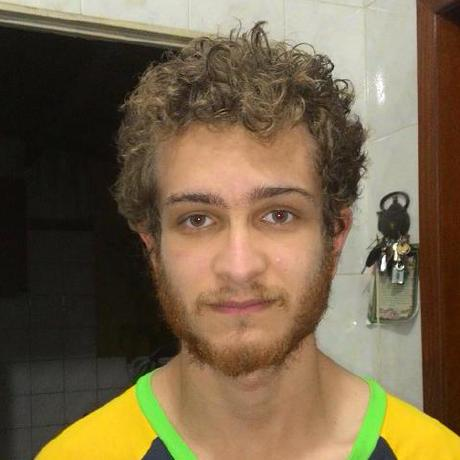
\includegraphics[width=\linewidth]{davidson}
						\caption{\scriptsize{Davidson Francis\\PUC Minas}}
					\end{subfigure}
					\quad
					\quad
					\begin{subfigure}{0.2\linewidth}
						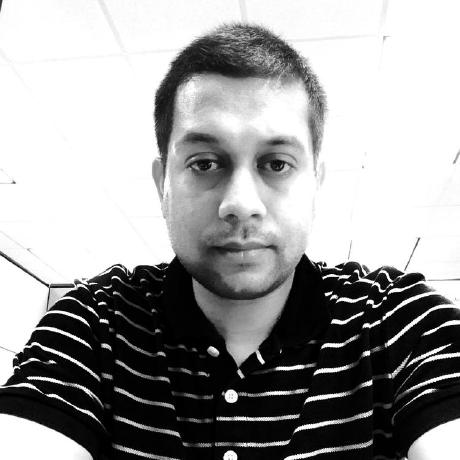
\includegraphics[width=\linewidth]{subhra}
						\caption{\scriptsize{Subhra Sarkar\\EchoStar Corp.}}
					\end{subfigure}
				\caption{People involved in the Nanvix Project.}
			\end{figure}
		\end{frame}

		\begin{frame}
		\frametitle{The Nanvix Operating System}
		\framesubtitle{Kernel Features}
			\begin{itemize}
			\setlength\itemsep{0.7em}
				\item POSIX compliant system call interface
				\item Unix System V architecture
				\item Non-preemptive kernel
				\item Time-sharing
				\item Multiprogramming
				\item Interprocess communication
				\item Virtual memory with swapping
				\item Minix file system
				\item Uniform device interface
			\end{itemize}
		\end{frame}

		\begin{frame}
		\frametitle{The Nanvix Operating System}
		\framesubtitle{User-Land Features}
			\begin{itemize}
			\setlength\itemsep{0.5em}
				\item Standard C Library
				\item Unix-like utilities

				\end{itemize}
				\begin{figure}
					\centering
					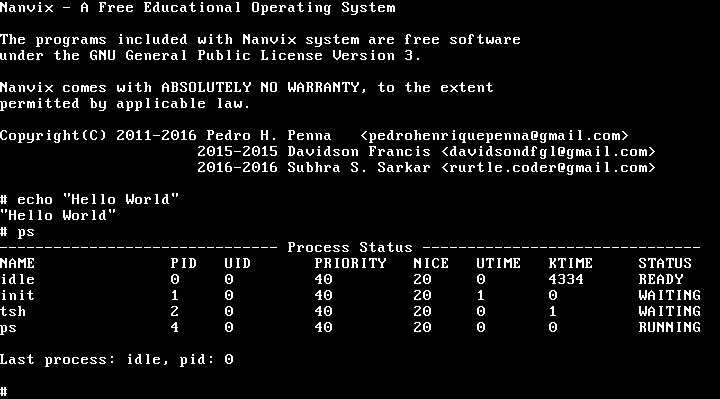
\includegraphics[width=0.8\textwidth]{nanvix}
					\caption{Nanvix running.}
				\end{figure}
		\end{frame}

\section{The Nanvix Kernel}

		\begin{frame}
		\frametitle{The Nanvix Operating System}
		\framesubtitle{Kernel Architecture}
			\begin{figure}
				\centering
				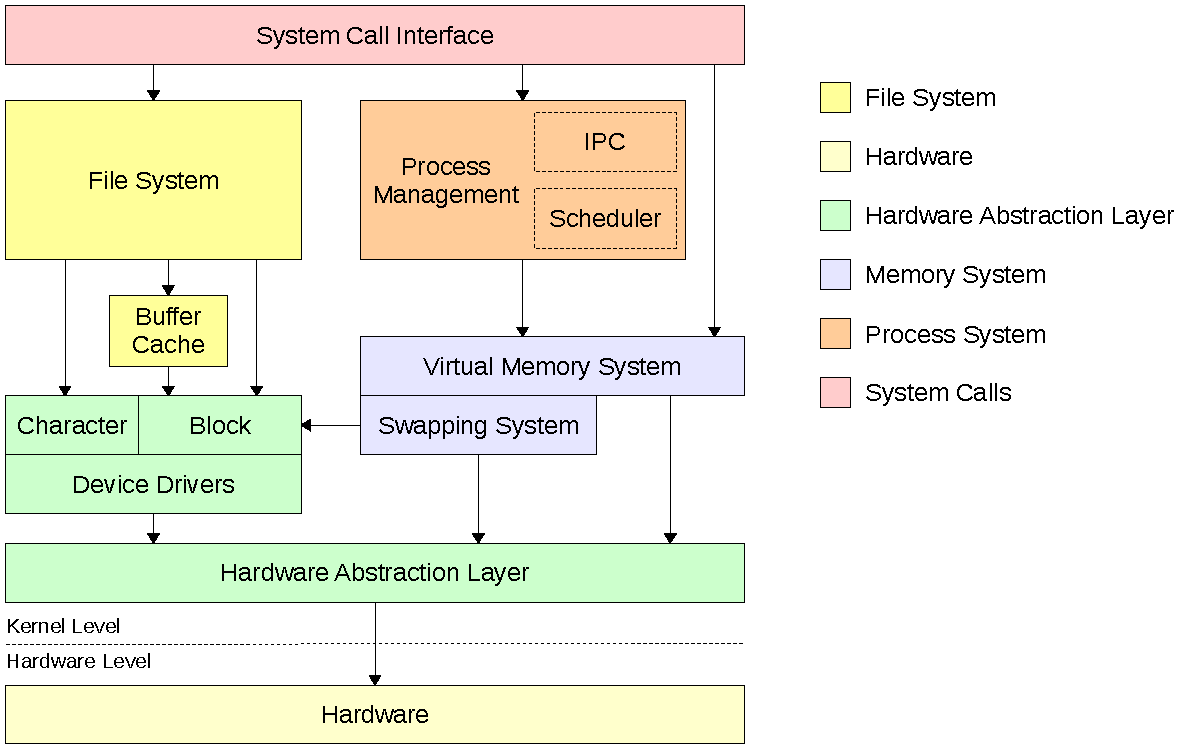
\includegraphics[width=\linewidth]{nanvix-architecture}
			\end{figure}
		\end{frame}

\section{Baby Steps}

		\begin{frame}
		\frametitle{The Nanvix Operating System}
		\framesubtitle{Source Tree}
			\begin{itemize}
			\setlength\itemsep{0.6em}
			\footnotesize
				\uncover<1->{
					\item \texttt{bin}: binaries
				}
				\uncover<2->{
					\item \texttt{doc}: documentation
				}
				\uncover<3->{
					\item \texttt{include}
					\begin{itemize}
					\setlength\itemsep{0.2em}
					\footnotesize
						\item \texttt{include/dev}: device drivers headers
						\item \texttt{include/fs}: file systems headers
						\item \texttt{include/i386}: platform-specific headers
						\item \texttt{include/nanvix}: kernel headers
					\end{itemize}
				}
				\uncover<4->{
					\item \texttt{lib}: libraries
				}
				\uncover<5->{
					\item \texttt{src} 
					\begin{itemize}
					\setlength\itemsep{0.2em}
					\footnotesize
						\item \texttt{src/kernel}: kernel sources
						\item \texttt{src/lib}: libraries sources
						\item \texttt{src/sbin}: superuser utilities sources
						\item \texttt{src/ubin}: user utilities sources
					\end{itemize}
				}
			\end{itemize}
		\end{frame}

	\begin{frame}[containsverbatim]
	\frametitle{The Nanvix Operating System}
	\framesubtitle{Building Development Tools}
	\begin{itemize}
	\setlength\itemsep{1.0em}
		\item Install required packets
	\begin{lstlisting}[language=bash,numbers=none,frame=single]
$ sudo apt-get install git make
	\end{lstlisting}

		\item Install useful (but not mandatory) packets
	\begin{lstlisting}[language=bash,numbers=none,frame=single]
$ sudo apt-get install tmux screen
	\end{lstlisting}

		\item Clone Nanvix repository
	\begin{lstlisting}[language=bash,numbers=none,frame=single]
$ cd ~
$ git clone https://github.com/nanvix/nanvix
$ cd ~/nanvix
	\end{lstlisting}
	\end{itemize}

	\end{frame}

	\begin{frame}[containsverbatim]
	\frametitle{The Nanvix Operating System}
	\framesubtitle{Building Development Tools}
	\begin{itemize}
	\setlength\itemsep{1.0em}
		\item Build cross-compiler (GCC and GNU Binutils)
	\begin{lstlisting}[language=bash,numbers=none,frame=single]
$ sudo bash tools/dev/setup-toolchain.sh
	\end{lstlisting}

		\item Install Bochs Emulator
	\begin{lstlisting}[language=bash,numbers=none,frame=single]
$ sudo bash tools/dev/setup-bochs.sh
	\end{lstlisting}

		\item Reboot O.S. (required to build Nanvix properly)

	\begin{lstlisting}[language=bash,numbers=none,frame=single]
$ sudo reboot now
	\end{lstlisting}

	\end{itemize}
	\end{frame}

	\begin{frame}[containsverbatim]
	\frametitle{The Nanvix Operating System}
	\framesubtitle{Building \& Running}
		\begin{itemize}
			\item Build the kernel and O.S. image
			\begin{lstlisting}[language=bash,numbers=none,frame=single]
$ make nanvix
$ make image
			\end{lstlisting}
		\end{itemize}

		\begin{itemize}
			\item Run Nanvix in normal (default) mode
				\begin{lstlisting}[language=bash,numbers=none,frame=single]
$ bash tools/run/run.sh
				\end{lstlisting}
		\end{itemize}

		\begin{itemize}
			\item Run Nanvix debug mode with GDB integration
				\begin{lstlisting}[language=bash,numbers=none,frame=single]
$ bash tools/run/run.sh --debug
				\end{lstlisting}
		\end{itemize}
	\end{frame}


	\begin{frame}[containsverbatim]
	\frametitle{The Nanvix Operating System}
	\framesubtitle{Building \& Running}
		\begin{figure}[t]
			\captionsetup[subfigure]{
				labelformat=empty}
				\begin{subfigure}{0.42\linewidth}
					\caption{\scriptsize{Nanvix}}
					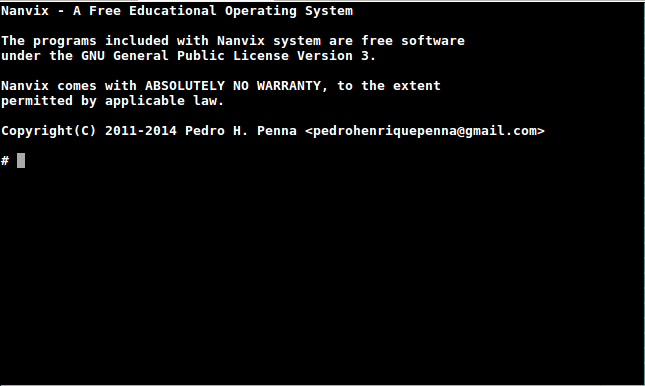
\includegraphics[width=\linewidth]{img/terminal-nanvix.png}
				\end{subfigure}
				\quad\quad\quad\quad
				\begin{subfigure}{0.42\linewidth}
					\caption{\scriptsize{GDB}}
					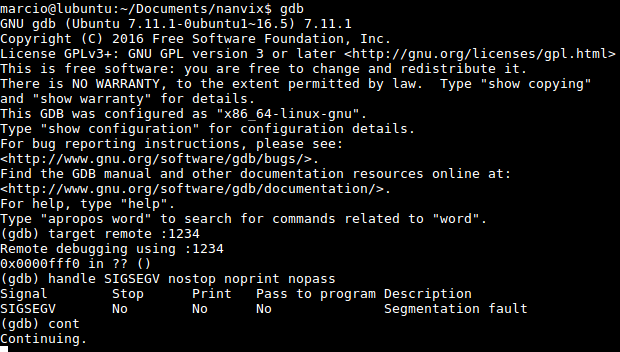
\includegraphics[width=\linewidth]{img/terminal-GDB.png}
				\end{subfigure}
		\end{figure}

		\begin{minipage}{.4\textwidth}
			\begin{lstlisting}[language=bash,numbers=none,frame=single,basicstyle=\tiny\ttfamily,]
$ bash tools/run/run.sh --debug
			\end{lstlisting}
		\end{minipage}
		\hfill
		\begin{minipage}{.48\textwidth}
			\begin{lstlisting}[language=bash,numbers=none,frame=single,basicstyle=\tiny\ttfamily,]
$ gdb
$ target remote :1234
$ handle SIGSEGV nostop noprint nopass
$ cont
			\end{lstlisting}
			
			{\scriptsize Load kernel symbol file:}
			\begin{lstlisting}[language=bash,numbers=none,frame=single,basicstyle=\tiny\ttfamily,]
$ symbol-file bin/kernel
			\end{lstlisting}

		\end{minipage}
	\end{frame}
	
\end{document}
